% -----------------------------*- LaTeX -*------------------------------
\documentclass[UTF8]{article}
% ------------------------------------------------------------------------
% Packages
% ------------------------------------------------------------------------
\usepackage{ctex} % 支持中文
\usepackage[body={7in, 9in},left=1in,right=1in]{geometry} % 改变页边距
\usepackage{amsmath} % AMS 的数学宏包
\usepackage{amsfonts} % AMS 的数学字体宏包
\usepackage{amssymb} % AMS 符号库
\usepackage{bm} % 数学公式中的黑斜体
\usepackage{amsthm} % AMS 的定理环境宏包
\usepackage{graphicx} % 插图
\usepackage{subfigure} % 插子图
\usepackage{nicefrac} % 好看的分数
\usepackage{mathrsfs} % mathscr font
\usepackage{caption} % caption
\usepackage{algorithm,algorithmicx} % 伪代码支持宏包
\usepackage[noend]{algpseudocode} % 伪代码
\usepackage{fancyhdr} % 设置页眉、页脚
\usepackage{adjustbox} % 图片尺寸自动调整
\usepackage{esint} % 积分符号
\usepackage{mathtools} % 数学宏包的重要补充
\usepackage{upgreek} % 数学环境的直立希腊字母
\usepackage{enumitem} % 使用enumitem宏包, 改变列表项的格式
\usepackage{color} % 支持彩色
\usepackage{extarrows} % 任意长度的箭头
\usepackage{tikz} % 绘图
\usepackage{forest} % 绘树
\usepackage{xcolor} % 颜色宏包
\usepackage{breqn} % 公式自动换行
\usepackage{fontsize} % 字体大小
\usepackage[framemethod=TikZ]{mdframed} % 给文字加框
\usepackage{fontspec} % 字体库
\usepackage{bigstrut} % 用于表格中的换行
\usepackage{multirow} % 表格中多行单元格合并
\usepackage{multicol} % 表格中多列单元格合并
\usepackage{longtable} % 长表格
\usepackage{rotating} % 旋转图形和表格      以上三者用于绘制三线表
\usepackage{booktabs} % 三线表宏包
\usepackage{scribe} % Scribe 模板
\usepackage{diagbox} % 表格斜线
\usepackage{listings} % 插入代码
\usepackage{hyperref} % 超链接
\usetikzlibrary{automata} % 引入automata库
\usetikzlibrary{shapes,arrows,positioning,chains} % 引入positioning库
% ------------------------------------------------------------------------
% Macros
% ------------------------------------------------------------------------
%~~~~~~~~~~~~~~~
% Utility latin
%~~~~~~~~~~~~~~~
\newcommand{\ie}{\textit{i.e.}}
\newcommand{\eg}{\textit{e.g.}}
%~~~~~~~~~~~~~~~
% Environment shortcuts
%~~~~~~~~~~~~~~~
\newcommand{\balign}[1]{\ealign{\begin{align}#1\end{align}}}
\newcommand{\baligns}[1]{\ealigns{\begin{align*}#1\end{align*}}}
\newcommand{\bitemize}[1]{\eitemize{\begin{itemize}#1\end{itemize}}}
\newcommand{\benumerate}[1]{\eenumerate{\begin{enumerate}#1\end{enumerate}}}
%~~~~~~~~~~~~~~~
% Text with quads around it
%~~~~~~~~~~~~~~~
\newcommand{\qtext}[1]{\quad\text{#1}\quad}
%~~~~~~~~~~~~~~~
% Shorthand for math formatting
%~~~~~~~~~~~~~~~
\newcommand{\mbb}[1]{\mathbb{#1}}
\newcommand{\mbi}[1]{\boldsymbol{#1}} % Bold and italic (math bold italic)
\newcommand{\mbf}[1]{\mathbf{#1}}
\newcommand{\mc}[1]{\mathcal{#1}}
\newcommand{\mrm}[1]{\mathrm{#1}}
\newcommand{\tbf}[1]{\textbf{#1}}
\newcommand{\tsc}[1]{\textsc{#1}}
%\def\\langle {{\langle }}
%\def\\rangle {{\rangle }}
\newcommand{\sT}{\sf T}
\newcommand{\grad}{\nabla}
\newcommand{\Proj}{\Pi}
%~~~~~~~~~~~~~~~
% Common sets 定义数集符号
%~~~~~~~~~~~~~~~
\newcommand{\R}{\mathbb{R}}
\newcommand{\Z}{\mathbb{Z}}
\newcommand{\Q}{\mathbb{Q}}
\newcommand{\N}{\mathbb{N}}
\newcommand{\C}{\mathbb{C}}
\newcommand{\reals}{\mathbb{R}} % Real number symbol
\newcommand{\integers}{\mathbb{Z}} % Integer symbol
\newcommand{\rationals}{\mathbb{Q}} % Rational numbers
\newcommand{\naturals}{\mathbb{N}} % Natural numbers
\newcommand{\complex}{\mathbb{C}} % Complex numbers
%~~~~~~~~~~~~~~~
% Common functions
%~~~~~~~~~~~~~~~
\renewcommand{\exp}[1]{\operatorname{exp}\left(#1\right)} % Exponential
\newcommand{\indic}[1]{\mbb{I}\left(#1\right)} % Indicator function
\newcommand{\indicsub}[2]{\mbb{I}_{#2}\left(#1\right)} % Indicator function
\newcommand{\argmax}{\mathop\mathrm{arg\, max}} % Defining math symbols
\newcommand{\argmin}{\mathop\mathrm{arg\, min}}
\renewcommand{\arccos}{\mathop\mathrm{arccos}}
\newcommand{\dom}{\mathop\mathrm{dom}} % Domain
\newcommand{\range}{\mathop\mathrm{range}} % Range
\newcommand{\diag}{\mathop\mathrm{diag}}
\newcommand{\tr}{\mathop\mathrm{tr}}
\newcommand{\abs}{\mathop\mathrm{abs}}
\newcommand{\card}{\mathop\mathrm{card}}
\newcommand{\sign}{\mathop\mathrm{sign}}
\newcommand{\prox}{\mathrm{prox}} % prox
\newcommand{\rank}[1]{\mathrm{rank}(#1)}
\newcommand{\supp}[1]{\mathrm{supp}(#1)}
\newcommand{\norm}[1]{\lVert#1\rVert}
%~~~~~~~~~~~~~~~
% Common probability symbols
%~~~~~~~~~~~~~~~
\newcommand{\family}{\mathcal{P}} % probability family / statistical model
\newcommand{\iid}{\stackrel{\mathrm{iid}}{\sim}}
\newcommand{\ind}{\stackrel{\mathrm{ind}}{\sim}}
\newcommand{\E}{\mathbb{E}} % Expectation symbol
\newcommand{\Earg}[1]{\E\left[#1\right]}
\newcommand{\Esubarg}[2]{\E_{#1}\left[#2\right]}
\renewcommand{\P}{\mathbb{P}} % Probability symbol
\newcommand{\Parg}[1]{\P\left(#1\right)}
\newcommand{\Psubarg}[2]{\P_{#1}\left[#2\right]}
%\newcommand{\Cov}{\mrm{Cov}} % Covariance symbol
%\newcommand{\Covarg}[1]{\Cov\left[#1\right]}
%\newcommand{\Covsubarg}[2]{\Cov_{#1}\left[#2\right]}
%\newcommand{\model}{\mathcal{P}} % probability family / statistical model
%~~~~~~~~~~~~~~~
% Distributions
%~~~~~~~~~~~~~~~
%\newcommand{\Gsn}{\mathcal{N}}
%\newcommand{\Ber}{\textnormal{Ber}}
%\newcommand{\Bin}{\textnormal{Bin}}
%\newcommand{\Unif}{\textnormal{Unif}}
%\newcommand{\Mult}{\textnormal{Mult}}
%\newcommand{\NegMult}{\textnormal{NegMult}}
%\newcommand{\Dir}{\textnormal{Dir}}
%\newcommand{\Bet}{\textnormal{Beta}}
%\newcommand{\Gam}{\textnormal{Gamma}}
%\newcommand{\Poi}{\textnormal{Poi}}
%\newcommand{\HypGeo}{\textnormal{HypGeo}}
%\newcommand{\GEM}{\textnormal{GEM}}
%\newcommand{\BP}{\textnormal{BP}}
%\newcommand{\DP}{\textnormal{DP}}
%\newcommand{\BeP}{\textnormal{BeP}}
%\newcommand{\Exp}{\textnormal{Exp}}
%~~~~~~~~~~~~~~~
% Theorem-like environments
%~~~~~~~~~~~~~~~
%\theoremstyle{definition}
%\newtheorem{definition}{Definition}
%\newtheorem{example}{Example}
%\newtheorem{problem}{Problem}
%\newtheorem{lemma}{Lemma}
%~~~~~~~~~~~~~~~
% 组合数学的模板和作业里用到的一些宏包和自定义命令
%~~~~~~~~~~~~~~~
\renewcommand{\emph}[1]{\begin{kaishu}#1\end{kaishu}}
\newcommand{\falfac}[1]{^{\underline{#1}}}
\newcommand{\binomfrac}[2]{\frac{#1^{\underline{#2}}}{#2!}}
\newcommand{\ceil}[1]{\left\lceil #1 \right\rceil}
\newcommand{\floor}[1]{\left\lfloor #1 \right\rfloor}
\newcommand{\suminfty}[2]{\sum_{#1=#2}^{\infty}}
\newcommand{\suminftyk}[0]{\sum_{k=0}^{\infty}}
\newcommand{\sumint}[3]{\sum_{#1=#2}^{#3}}
\newcommand{\sumintk}[2]{\sum_{k=#1}^{#2}}
\newcommand{\suminti}[2]{\sum_{i=#1}^{#2}}
%~~~~~~~~~~~~~~~
% 定义新命令
%~~~~~~~~~~~~~~~
\newcommand*{\unit}[1]{\mathop{}\!\mathrm{#1}}
\newcommand*{\dif}{\mathop{}\!\mathrm{d}}%微分算子 d
\newcommand*{\pdif}{\mathop{}\!\partial}%偏微分算子
\newcommand*{\cdif}{\mathop{}\!\nabla}%协变导数、nabla 算子
\newcommand*{\laplace}{\mathop{}\!\Delta}%laplace 算子
\newcommand*{\deri}[1]{\mathrm{d} #1}
\newcommand*{\deriv}[2]{\frac{\mathrm{d} #1}{\mathrm{d} {#2}}}
\newcommand*{\derivh}[3]{\frac{\mathrm{d}^{#1} #2}{\mathrm{d} {#3^{#1}}}}
\newcommand*{\pderiv}[2]{\frac{\partial #1}{\partial {#2}}}
\newcommand*{\pderivh}[3]{\frac{\partial^{#1} #2}{\partial {#3^{#1}}}}
\newcommand*{\dderiv}[2]{\dfrac{\mathrm{d} #1}{\mathrm{d} {#2}}}
\newcommand*{\dderivh}[3]{\dfrac{\mathrm{d}^{#1} #2}{\mathrm{d} {#3^{#1}}}}
\newcommand*{\dpderiv}[2]{\dfrac{\partial #1}{\partial {#2}}}
\newcommand*{\dpderivh}[3]{\dfrac{\partial^{#1} #2}{\partial {#3^{#1}}}}
\newcommand{\me}[1]{\mathrm{e}^{#1}}%e 指数
\newcommand{\mi}{\mathrm{i}}%虚数单位
%\newcommand{\mc}{\mathrm{c}}%光速 定义与mathcal冲突
\newcommand{\red}[1]{\textcolor{red}{#1}}
\newcommand{\blue}[1]{\textcolor{blue}{#1}}
%\newcommand{\Rome}[1]{\setcounter{rome}{#1}\Roman{rome}}
%~~~~~~~~~~~~~~~
% 公式环境中箭头符号的简写
%~~~~~~~~~~~~~~~
\newcommand{\ra}{\rightarrow}
\newcommand{\Ra}{\Rightarrow}
\newcommand{\la}{\leftarrow}
\newcommand{\La}{\Leftarrow}
\newcommand{\lra}{\leftrightarrow}
\newcommand{\Lra}{\Leftrightarrow}
\newcommand{\lgla}{\longleftarrow}
\newcommand{\Lgla}{\Longleftarrow}
\newcommand{\lgra}{\longrightarrow}
\newcommand{\Lgra}{\Longrightarrow}
\newcommand{\lglra}{\longleftrightarrow}
\newcommand{\Lglra}{\Longleftrightarrow}
%~~~~~~~~~~~~~~~
% 一些数学的环境设置
%~~~~~~~~~~~~~~~
%\newcounter{counter_exm}\setcounter{counter_exm}{1}
%\newcounter{counter_prb}\setcounter{counter_prb}{1}
%\newcounter{counter_thm}\setcounter{counter_thm}{1}
%\newcounter{counter_lma}\setcounter{counter_lma}{1}
%\newcounter{counter_dft}\setcounter{counter_dft}{1}
%\newcounter{counter_clm}\setcounter{counter_clm}{1}
%\newcounter{counter_cly}\setcounter{counter_cly}{1}
\newtheorem{theorem}{{\hskip 1.7em \bf 定理}}
\newtheorem{lemma}[theorem]{\hskip 1.7em 引理}
\newtheorem{proposition}[theorem]{\hskip 1.7em 命题}
\newtheorem{claim}[theorem]{\hskip 1.7em 断言}
\newtheorem{corollary}[theorem]{\hskip 1.7em 推论}
% \newcommand{\problem}[1]{{\setlength{\parskip}{10pt}\noindent \bf{#1}}}
\newenvironment{solution}{{\noindent \bf 解 \quad}}{}
\newenvironment{remark}{{\noindent \bf 注 \quad}}{}
\newenvironment{definition}{{\noindent \bf 定义 \quad}}{}
\renewenvironment{proof}{{\setlength{\parskip}{7pt}\noindent\hskip 2em \bf 证明 \quad}}{\hfill$\qed$\par}
\newenvironment{example}{{\noindent\bf 例 \quad}}{\hfill$\qed$\par}
%\newenvironment{concept}[1]{{\bf #1\quad} \begin{kaishu}} {\end{kaishu}\par}
%~~~~~~~~~~~~~~~
% 本.tex文档中特殊定义命令
%~~~~~~~~~~~~~~~
\newcommand{\lno}[1]{\overline{#1}}
\newcommand{\NP}{\mathrm{NP}}
\newcommand{\coNP}{\mathrm{coNP}}
% \newcommand{\ISO}{\mathrm{ISO}}
\newcommand{\SAT}{\mathrm{SAT}}
\newcommand{\USAT}{\mathrm{USAT}}
% \newcommand{\threeSAT}{\mathrm{3\text{-}SAT}}
\renewcommand{\P}{\mathrm{P}}
% \mathchardef\mhyphen="2D
% \newcommand{\CNF}{\mathrm{CNF}}
% \newcommand{\DNF}{\mathrm{DNF}}
% \newcommand{\SetSp}{\mathrm{SET\text{-}SPLITTING}}
% \newcommand{\PUZZLE}{\mathrm{PUZZLE}}
% \newcommand{\SPATH}{\mathrm{SPATH}}
% \newcommand{\LPATH}{\mathrm{LPATH}}
% \newcommand{\UHAMPATH}{\mathrm{UHAMPATH}}
\newcommand{\SPACE}{\mathrm{SPACE}}
\newcommand{\NSPACE}{\mathrm{NSPACE}}
\newcommand{\PSPACE}{\mathrm{PSPACE}}
\newcommand{\NPSPACE}{\mathrm{NPSPACE}}
\newcommand{\DFA}{\mathrm{DFA}}
\newcommand{\NFA}{\mathrm{NFA}}
\newcommand{\TQBF}{\mathrm{TQBF}}
% \newcommand{\L}{\mathrm{L}}
\renewcommand{\O}{\mathrm{O}}
\newcommand{\NL}{\mathrm{NL}}
\newcommand{\coNL}{\mathrm{coNL}}
\newcommand{\LADDER}{\mathrm{LADDER_{DFA}}}
\newcommand{\hd}{\mathrm{\text{-}hard}}
\newcommand{\ADD}{\mathrm{ADD}}
\newcommand{\STCN}{\mathrm{STRONGLY\text{-}CONNECTED}}
\newcommand{\PATH}{\mathrm{PATH}}
\newcommand{\A}{\mathrm{A}}
%使用align环境公式换页
\allowdisplaybreaks[4]

\definecolor{dkgreen}{rgb}{0,0.6,0}
\definecolor{gray}{rgb}{0.5,0.5,0.5}
\definecolor{mauve}{rgb}{0.58,0,0.82}
\lstset{
  frame=tb,
  aboveskip=3mm,
  belowskip=3mm,
  showstringspaces=false,
  columns=flexible,
  framerule=1pt,
  rulecolor=\color{gray!35},
  backgroundcolor=\color{gray!5},
  basicstyle={\small\ttfamily},
  numbers=none,
  numberstyle=\tiny\color{gray},
  keywordstyle=\color{blue},
  commentstyle=\color{dkgreen},
  stringstyle=\color{mauve},
  breaklines=true,
  breakatwhitespace=true,
  tabsize=3,
}

\setmainfont{Times New Roman}
\setsansfont{Times New Roman}
\setmonofont{Menlo}
\setCJKmainfont{STHeiti}
\setCJKsansfont{STSong}
\setCJKmonofont{STFangsong}
\punctstyle{kaiming}

\begin{document}

\pagestyle{fancy}
\lhead{\emph{操作系统实例分析}}
\chead{\emph{中国科学院大学}}
\rhead{\emph{张家玮、罗彦博、赵逸鸣}}

\begin{center}
    {\LARGE \bf 实例分析1:进程}
\end{center}

\section{第零部分:初识xv6}

\subsection{基础题}

\begin{enumerate}
    \item 安装相应工具链,在 qemu 中运行 xv6。并在操作系统中运行 ls 命令。
    
    我使用的是MacBook,在qemu中运行xv6需要在终端中依次输入以下命令:

    \begin{lstlisting}[language=bash]
      brew tap riscv/riscv # 添加riscv工具链
      brew install riscv-tools qemu # 安装riscv工具链和qemu
      git clone https://github.com/mit-pdos/xv6-riscv.git
      cd xv6-riscv
      make # 编译xv6
      make qemu # 在qemu中运行xv6
    \end{lstlisting}

    现场演示make与ls命令。

    \item 阅读 ls.c 。请回答: 代码中的 \texttt{read()} 函数和 \texttt{printf()} 函数哪个是系统调用?它们的函数声明在哪里,函数定义在哪里?
    
    \texttt{read()}是系统调用,函数声明在user/user.h中:
    
    \begin{lstlisting}[language=C]
      // system calls
      int read(int, void*, int);
    \end{lstlisting}
    
    定义在user/usys.pl中,它定义了一个\texttt{entry}子程序,并且依次为多个系统调用生成相应的汇编代码(这里只展示了\texttt{read}):

    \begin{lstlisting}[language=perl]
      sub entry {
        my $name = shift;
        print ".global $name\n"; # 定义一个全局符号,以便其他文件可以访问该系统调用
        print "${name}:\n"; # 定义一个标签,以便其他文件可以调用该系统调用
        print " li a7, SYS_${name}\n"; # 将系统调用号送给a7
        print " ecall\n"; # 进入内核态发起系统调用
        print " ret\n"; # 返回至调用点
      }

      entry("read"); # 生成read系统调用的汇编代码
    \end{lstlisting}

    所生成的汇编代码在user/usys.S中:

    \begin{lstlisting}[language=s]
      .global read
      read:
       li a7, SYS_read
       ecall
       ret
    \end{lstlisting}    

    \texttt{printf()}不是系统调用,函数声明在user/user.h中,定义在user/printf.c中。

    声明如下:

    \begin{lstlisting}[language=C]
      // ulib.c
      void printf(const char*, ...) __attribute__ ((format (printf, 1, 2))); // __attribute__ ((format (printf, 1, 2))) 用于指定函数的格式属性。它让编译器在编译时检查 printf 函数的调用,确保传入的格式字符串和参数类型匹配
    \end{lstlisting}

    定义就不复制过来了。

    \item 阅读 usys.S ,查阅 RISC-V 相关知识,请问 ecall 指令的功能是什么?(如果找不到usys.S ,请自我反思一下,不要阅读静态代码)
    
    usys.S是由usys.pl生成的!如果不进行编译,usys.S自然找不到。在Makefile中,生成usys.S的代码如下:

    \begin{lstlisting}[language=make]
      $U/usys.S : $U/usys.pl
          perl $U/usys.pl > $U/usys.S
    \end{lstlisting}

    ecall指令是在RISCV中被定义为环境调用指令,用于向系统发起一次系统调用。当执行到ecall指令时,根据a7寄存器的值来确定系统调用的类型,从用户态切换到内核态,执行对应的系统调用,然后返回继续执行用户程序。
\end{enumerate}

\subsection{进阶题}

\noindent
阅读 xv6 项目相关的 Makefile 文件、mkfs.c 文件和链接器相关文件,分析 xv6 把内核和用户态程序编译链接的整个过程。并思考一个问题,xv6运行的时候,ls 可以看到里面有一个 README 文件,我在 xv6 操作系统把它删除,为什么本地项目的 README 文件仍存在 (反之如此)?

\vspace{1em}

xv6的Makefile文件中定义了编译xv6的规则,先指定\texttt{OBJS},即所有的目标文件,再指定编译器(\texttt{CC})、汇编器(\texttt{AS})、链接器(\texttt{LD})、编译选项(\texttt{CFLAGS})等,再链接内核目标、编译用户程序、最后使用mkfs生成文件系统镜像,包括 README 文件和用户程序。

在运行xv6时,会将镜像文件加载到内存中,因此,xv6运行的时候,ls可以看到里面有一个README文件,如果在xv6操作系统中删除README文件,本地项目的README文件仍然存在,是因为本地项目的README文件和xv6的文件系统镜像文件是两个不同的文件,删除xv6的文件系统镜像文件中的README文件并不会影响本地项目的README文件。

\newpage
\section{第四部分: 进程的运行}

\subsection{基础题}

\begin{enumerate}
    \item proc.c 中 \texttt{uchar initcode[]} 的诡异的二进制数据的含义是什么?为什么 \texttt{userinit()} 函数要把它拷贝到 user page 中?它和 user/initCode.S 有什么联系?
    
    \begin{lstlisting}[language=C]
        // a user program that calls exec("/init")
        // assembled from ../user/initcode.S
        // od -t xC ../user/initcode
        uchar initcode[] = {
          0x17, 0x05, 0x00, 0x00, 0x13, 0x05, 0x45, 0x02,
          0x97, 0x05, 0x00, 0x00, 0x93, 0x85, 0x35, 0x02,
          0x93, 0x08, 0x70, 0x00, 0x73, 0x00, 0x00, 0x00,
          0x93, 0x08, 0x20, 0x00, 0x73, 0x00, 0x00, 0x00,
          0xef, 0xf0, 0x9f, 0xff, 0x2f, 0x69, 0x6e, 0x69,
          0x74, 0x00, 0x00, 0x24, 0x00, 0x00, 0x00, 0x00,
          0x00, 0x00, 0x00, 0x00
        };        
    \end{lstlisting}
    
    这一些二进制数据实际上拼起来是一个用户程序,调用\texttt{exec("/init")}。
    
    \texttt{userinit()}函数将这个用户程序拷贝到用户页中,意在用户态执行此进程,并实现进程隔离。
    
    下面展示出userinit()函数的代码:

    \begin{lstlisting}[language=C]
        // Set up first user process.
        void
        userinit(void)
        {
          struct proc *p;
        
          p = allocproc();
          initproc = p;
          
          // allocate one user page and copy initcode's instructions
          // and data into it.
          uvmfirst(p->pagetable, initcode, sizeof(initcode));
          p->sz = PGSIZE;
        
          // prepare for the very first "return" from kernel to user.
          p->trapframe->epc = 0;      // user program counter
          p->trapframe->sp = PGSIZE;  // user stack pointer
        
          safestrcpy(p->name, "initcode", sizeof(p->name));
          p->cwd = namei("/");
        
          p->state = RUNNABLE;
        
          release(&p->lock);
        }
    \end{lstlisting}

    \texttt{initcode[]}和user/initCode.S是一样的,都是一个用户程序,调用\texttt{exec("/init")}。

    \item 第一个进程启动后在用户态执行的程序是什么?这个程序执行了哪个系统调用?
    
    第一个进程启动后在用户态执行的程序是user/init.c,代码如下:

    \begin{lstlisting}[language=C]
        // init: The initial user-level program

        #include "kernel/types.h"
        #include "kernel/stat.h"
        #include "kernel/spinlock.h"
        #include "kernel/sleeplock.h"
        #include "kernel/fs.h"
        #include "kernel/file.h"
        #include "user/user.h"
        #include "kernel/fcntl.h"
        
        char *argv[] = { "sh", 0 };
        
        int
        main(void)
        {
          int pid, wpid;
        
          if(open("console", O_RDWR) < 0){
            mknod("console", CONSOLE, 0);
            open("console", O_RDWR);
          }
          dup(0);  // stdout
          dup(0);  // stderr
        
          for(;;){
            printf("init: starting sh\n");
            pid = fork();
            if(pid < 0){
              printf("init: fork failed\n");
              exit(1);
            }
            if(pid == 0){
              exec("sh", argv);
              printf("init: exec sh failed\n");
              exit(1);
            }
        
            for(;;){
              // this call to wait() returns if the shell exits,
              // or if a parentless process exits.
              wpid = wait((int *) 0);
              if(wpid == pid){
                // the shell exited; restart it.
                break;
              } else if(wpid < 0){
                printf("init: wait returned an error\n");
                exit(1);
              } else {
                // it was a parentless process; do nothing.
              }
            }
          }
        }
    \end{lstlisting}
    
    这个程序执行了open()、mknod()、dup()、fork()、exec()、wait()、exit()等系统调用。

    open() 系统调用用于打开文件,mknod() 系统调用用于创建设备文件,dup() 系统调用用于复制文件描述符,fork() 系统调用用于创建子进程,exec() 系统调用用于执行程序,wait() 系统调用用于等待子进程退出,exit() 系统调用用于退出进程。

    上面的程序是一个无限循环,不断创建子进程执行sh程序,如果sh程序退出,则重新创建一个sh进程。

    \item 在 exec.c 的 exec() 中,用到的 struct elfhdr 数据结构,其中 magic , phnum,phoff 等字段的作用是什么?以及 struct proghdr 的数据结构,其中 vaddr,memsz,filesz 等字段的作用是什么?
    
    struct elfhdr 数据结构是ELF文件头,用于描述ELF文件的基本信息,magic字段用于标识ELF文件,即所有ELF文件的开头都是0x464C457F("\textbackslash x7FELF"的小端序),phnum字段表示ELF文件中的程序头的数量,phoff字段表示ELF文件中的程序头表的偏移量。

    struct proghdr 数据结构是程序头,用于描述ELF文件中的程序段的信息,vaddr字段表示程序段的虚拟地址,memsz字段表示程序段在内存中的大小,filesz字段表示程序段在文件中的大小。

    \item 在 exec() 中,如何确定并设置待运行的程序的 PC 值和栈指针?
    
    首先需要弄清楚exec()函数的两个参数意义:

    \begin{lstlisting}[language=C]
      int
      exec(char *path, char **argv)
    \end{lstlisting}
    
    \texttt{path}是要执行的程序的路径,\texttt{argv}是命令行参数,于是\texttt{exec()}函数的主要工作是将\texttt{path}指定的程序加载到内存中并替换当前进程的地址空间,然后开始执行新程序。
    
    \texttt{exec()} 函数会读取 ELF 文件头,以获取程序入口点的地址,然后将这个地址设置为新进程的 PC 值,即:

    \begin{lstlisting}[language=C]
      p->trapframe->epc = elf.entry;  // initial program counter = main
    \end{lstlisting}

    在加载完程序段后,\texttt{exec()} 函数会为用户栈分配内存,并将命令行参数拷贝到栈中。然后,计算并设置栈指针(SP)。计算过程如下:

    \begin{lstlisting}[language=C]
        // Push argument strings, prepare rest of stack in ustack.
        for(argc = 0; argv[argc]; argc++) {
          if(argc >= MAXARG)
            goto bad;
          sp -= strlen(argv[argc]) + 1; // including '\0'
          sp -= sp % 16; // riscv sp must be 16-byte aligned
          if(sp < stackbase)
            goto bad;
          if(copyout(pagetable, sp, argv[argc], strlen(argv[argc]) + 1) < 0)
            goto bad;
          ustack[argc] = sp;
        }
        ustack[argc] = 0;
        
        // push the array of argv[] pointers.
        sp -= (argc+1) * sizeof(uint64); 
        sp -= sp % 16;
        if(sp < stackbase)
          goto bad;
        if(copyout(pagetable, sp, (char *)ustack, (argc+1)*sizeof(uint64)) < 0)
          goto bad;

        p->trapframe->sp = sp; // initial stack pointer
    \end{lstlisting}

    \item exec() 执行完以后,返回的地址是什么?为什么?
    
    exec() 函数执行完以后,返回的地址是新程序的入口点地址elf.entry,因为它会用新程序替换当前进程的地址空间,并开始执行新程序。
    
    \item 在user/init.c 中调用了 fork() 函数创建子进程。请问在调用 fork() 系统调用后,是父
    进程先返回还是子进程先返回?

    子进程先返回,因为父进程会wait()子进程,等待子进程退出。

    \item 在调用 fork() 系统调用后,子进程是如何从 RUNNABLE 转换到 RUNNING 状态的?
    
    实际上,子进程是由操作系统调度器调度的,当子进程创建后,fork()函数会将子进程的状态设置为RUNNABLE,然后由操作系统调度器调度,将子进程从RUNNABLE状态转换到RUNNING状态。

    \item 对于父进程和子进程, fork() 返回的 pid 相同么?为什么?
  
    父进程和子进程是两个不同的进程,pid当然不同。具体关注代码来说,fork()函数的返回值是allocproc()函数分配的新进程的pid,而这个pid是从1开始递增的,所以父进程和子进程的pid是不同的。代码如下:

    \begin{lstlisting}[language=C]
      int nextpid = 1;

      int
      allocpid()
      {
        int pid;
        
        acquire(&pid_lock);
        pid = nextpid;
        nextpid = nextpid + 1;
        release(&pid_lock);

        return pid;
      }
    \end{lstlisting}

    \item wait 系统调用的功能?
    
    wait()系统调用用于等待子进程退出,如果子进程已经退出,则wait()会立即返回,否则wait()会阻塞当前进程,直到子进程退出。
\end{enumerate}

\subsection{进阶题}

\noindent
请结合代码详细分析 Linux 中 elf 文件格式(利用 readelf 命令),以及链接和加载的机制。

\vspace{1em}

在kernel/elf.h中定义了ELF文件头的数据结构elfhdr和程序头的数据结构proghdr,代码如下:

\begin{lstlisting}[language=C]
    // Format of an ELF executable file

    #define ELF_MAGIC 0x464C457FU  // "\x7FELF" in little endian
    
    // File header
    struct elfhdr {
      uint magic;  // must equal ELF_MAGIC
      uchar elf[12];
      ushort type;
      ushort machine;
      uint version;
      uint64 entry;
      uint64 phoff;
      uint64 shoff;
      uint flags;
      ushort ehsize;
      ushort phentsize;
      ushort phnum;
      ushort shentsize;
      ushort shnum;
      ushort shstrndx;
    };
    
    // Program section header
    struct proghdr {
      uint32 type;
      uint32 flags;
      uint64 off;
      uint64 vaddr;
      uint64 paddr;
      uint64 filesz;
      uint64 memsz;
      uint64 align;
    };
\end{lstlisting}

elf文件格式的示意图如下所示:

\begin{figure}[H]
    \centering
    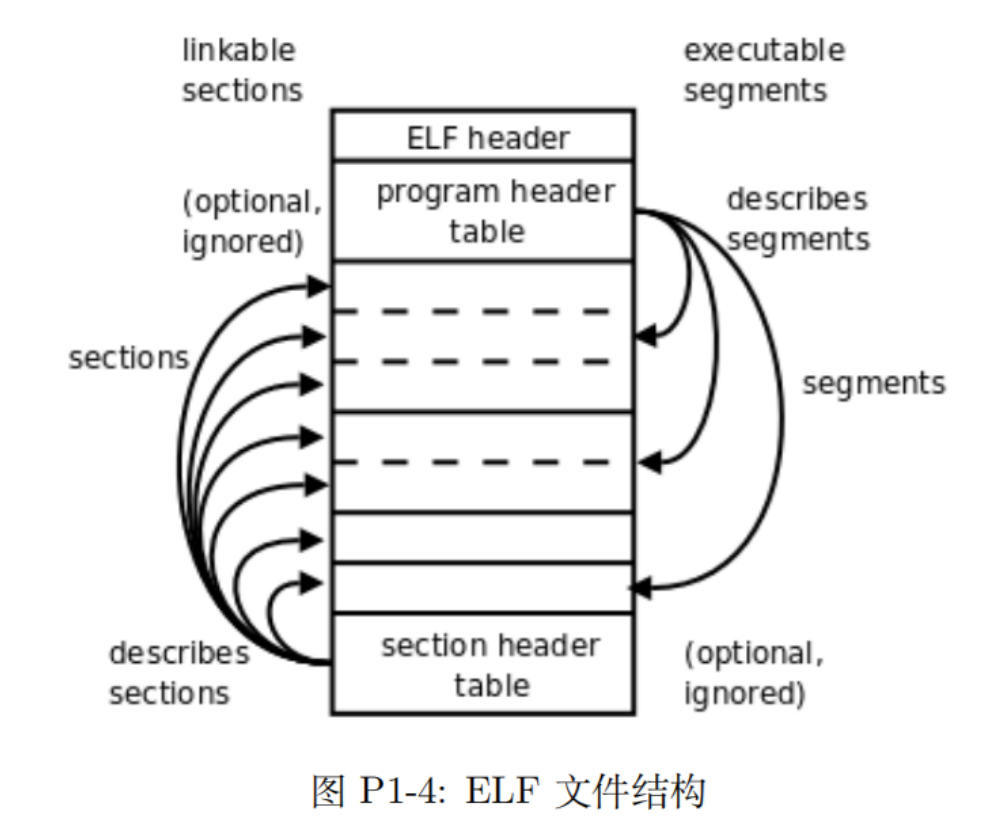
\includegraphics[width=0.6\textwidth]{elfformat2.jpg}
\end{figure}

随便写了一个汇编文件,编译之后得到可执行文件,然后使用readelf命令查看可执行文件的信息,如下所示:

\begin{lstlisting}[language=bash]
  readelf -h hello
\end{lstlisting}

输出如下:

\begin{lstlisting}
ELF Header:
  Magic:   7f 45 4c 46 02 01 01 00 00 00 00 00 00 00 00 00 
  Class:                             ELF64
  Data:                              2's complement, little endian
  Version:                           1 (current)
  OS/ABI:                            UNIX - System V
  ABI Version:                       0
  Type:                              EXEC (Executable file)
  Machine:                           RISC-V
  Version:                           0x1
  Entry point address:               0x100e8
  Start of program headers:          64 (bytes into file)
  Start of section headers:          944 (bytes into file)
  Flags:                             0x4, double-float ABI
  Size of this header:               64 (bytes)
  Size of program headers:           56 (bytes)
  Number of program headers:         3
  Size of section headers:           64 (bytes)
  Number of section headers:         7
  Section header string table index: 6
\end{lstlisting}

\begin{lstlisting}[language=bash]
  readelf -l hello
\end{lstlisting}

输出如下:

\begin{lstlisting}
  Elf file type is EXEC (Executable file)
  Entry point 0x100e8
  There are 3 program headers, starting at offset 64
  
  Program Headers:
    Type           Offset             VirtAddr           PhysAddr
                   FileSiz            MemSiz              Flags  Align
    RISCV_ATTRIBUT 0x0000000000000117 0x0000000000000000 0x0000000000000000
                   0x000000000000004c 0x0000000000000000  R      0x1
    LOAD           0x0000000000000000 0x0000000000010000 0x0000000000010000
                   0x000000000000010c 0x000000000000010c  R E    0x1000
    LOAD           0x000000000000010c 0x000000000001110c 0x000000000001110c
                   0x000000000000000b 0x000000000000000b  RW     0x1000
  
   Section to Segment mapping:
    Segment Sections...
     00     .riscv.attributes 
     01     .text 
     02     .data
\end{lstlisting}

链接是将多个目标文件和库文件组合成一个可执行文件的过程。链接可以分为两种类型:静态链接和动态链接。

静态链接(Static Linking):在编译时,将所有需要的库函数和目标文件组合到一个单一的可执行文件中。

动态链接(Dynamic Linking):在运行时,将库函数动态加载到内存中,并链接到可执行文件。

链接的过程包括以下几个步骤:

\begin{enumerate}
  \item 符号解析:链接器需要解析所有目标文件和库文件中的符号。符号可以是变量、函数或其他标识符。链接器需要确保每个符号都有唯一的定义,并且所有引用都能找到对应的定义。
  \item 重定位:链接器需要调整目标文件中的地址,以便它们在最终的可执行文件中正确指向。重定位包括调整代码和数据段中的地址,以反映它们在内存中的最终位置。
  \item 合并段:链接器将多个目标文件中的相同类型的段(如代码段、数据段)合并到一个段中。这样可以减少内存碎片,并提高程序的加载效率。
  \item 生成最终的可执行文件:链接器将所有目标文件和库文件合并,生成最终的可执行文件。这个文件包含所有代码和数据段,并且所有符号和地址都已正确解析和调整。
\end{enumerate}

加载是加载器将可执行文件从磁盘加载到内存中,并准备执行的过程。包括以下步骤:

\begin{enumerate}
  \item 读取可执行文件头:加载器首先读取可执行文件的头部信息,以确定文件格式、入口点、段信息等。
  \item 分配内存:根据可执行文件的段信息,加载器在内存中分配相应的空间,包括代码段、数据段、堆和栈。
  \item 加载段:将可执行文件的各个段(如代码段、数据段)加载到分配的内存区域中。
  \item 动态链接(如果使用动态链接):加载器在运行时加载动态库,并解析符号表,将库函数链接到可执行文件中。
  \item 设置入口点:加载器将程序计数器(PC)设置为可执行文件的入口点地址。
  \item 开始执行:加载器将控制权交给可执行文件,开始执行程序。
\end{enumerate}
\end{document}